\documentclass[12pt]{article}

\usepackage{graphicx}
\usepackage[sorting=none]{biblatex}
\usepackage[margin=1in]{geometry}
\usepackage[colorlinks=true]{hyperref}
\usepackage{amsmath}
\usepackage{amssymb}
\usepackage[format=plain, labelfont=it, font=footnotesize, labelsep=period]{caption}

\addbibresource{references.bib}

\title{Pendulum Lab Report 1}
\author{Kevin (Zerui) Wang}
\date{\today}

\begin{document}

\pagenumbering{gobble}

\maketitle

\pagenumbering{arabic}

\section{Introduction}
The first part of this lab report focuses on the relationship the period and release angle of a simple pendulum. After results were collected and analyzed, an improved version of the pendulum was created to collect angular data in order to determine the Q factor.

\section{Background} \label{Background}
For a simple pendulum with a mass $m$ hanging from a string with length $L$ experiencing a downwards force due to gravity $g$, the period, for a release angle $\theta$, is given by the following equation \cite{the-simple-pendulum}:
\begin{equation} \label{eq:eq1}
    2\pi \sqrt{\frac{L}{g}}
\end{equation}

This is otherwise known as the small angle approximation of a pendulum, which only holds if $\theta \lesssim 20^{\circ}$ \cite{the-simple-pendulum} (This phenomena may be observed if one were to release the pendulum from a large $\theta$). For $\theta \gtrsim 20^{\circ}$, a new model must be created to take into account the realistic behaviour of a pendulum, namely a second order differential equation with respect to $\theta$:
\begin{equation} \label{eq:eq2}
    \frac{d^2\theta}{dt^2} + \frac{g}{L}\sin{\theta} = 0
\end{equation}
which must be solved numerically where the solution to Equation \ref{eq:eq2} diverges from simple harmonic motion that could accurately predict the motion of a pendulum under small angle approximation \cite{the-simple-pendulum}. It may also be useful to note that the $m$ term does not come up in any of these equations, which implies pendulum period does not depend on mass.

Additionally the existence of air resistance and friction within the string fibres will cause a dampening effect on the oscillation of a pendulum. This effect can be modeled given an initial angle $\theta_0$ in radians, decay constant $\tau$, a pendulum period $T$, and a angular phase shift $\phi_0$ \cite{damped-oscillations}:
\begin{equation} \label{eq:eq3}
    \theta(t) = \theta_0 e^{-{t/\tau}} \cos\left(2\pi\frac{t}{T} + \phi_0\right)
\end{equation}

In order to quantify the dampening effect of a pendulum, its Q factor may be used, defined as follows for a damped oscillator \cite{pnp-physics}:
\begin{equation} \label{eq:eq4}
    Q = \pi\frac{\tau}{T}
\end{equation}
Another way of measuring the Q factor is counting the number of oscillation it takes for the amplitude to decay to $e^{-\pi} \approx 4\%$, or measuring $Q/n$ where the amplitude decays to $e^{-{\pi/n}}$ its original.

This way of determining the Q factor works because when $Q = n\pi\frac{\tau}{T}$, $t = \frac{QT}{n}$. The amplitude would them be $e^{-{t/T}} = e^{-{\pi/n}}$

\section{Period and Release Angle}

\subsection{Experimental Setup}
The initial setup for the pendulum was made by first attaching a protractor on a desk. The pendulum, made by tying a piece of cotton string around a stainless steel quick link, was then placed at the center of the protractor. The length of the pendulum was measured using measuring tape. An image of the experimental setup is shown below:

\begin{figure}[!hptb]
    \centering
    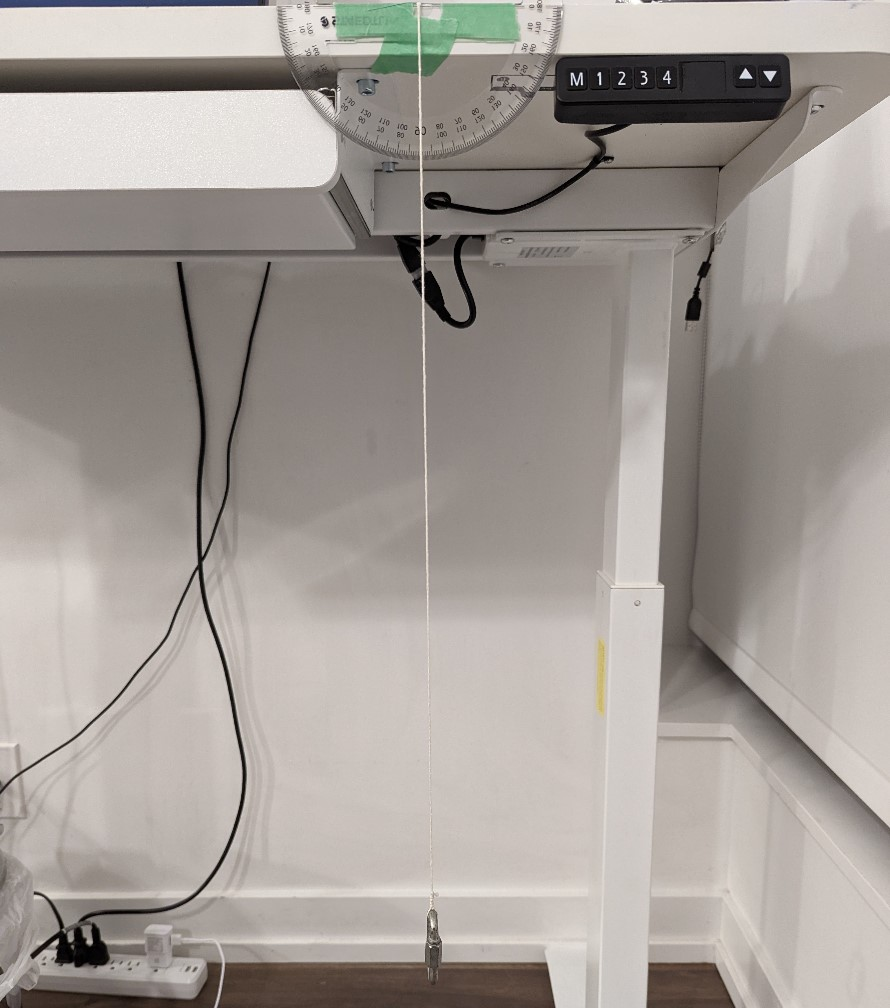
\includegraphics[width=0.5\textwidth]{../figures/exp_setup1.jpg}
    \caption{\centering Picture of experimental setup for period vs. release angle data collection}
    \label{fig:figure 1}
\end{figure}

\newpage

\subsection{Data}
The data collected for the period vs. release angle graph is shown in the plot below:

\begin{figure}[!hptb]
    \centering
    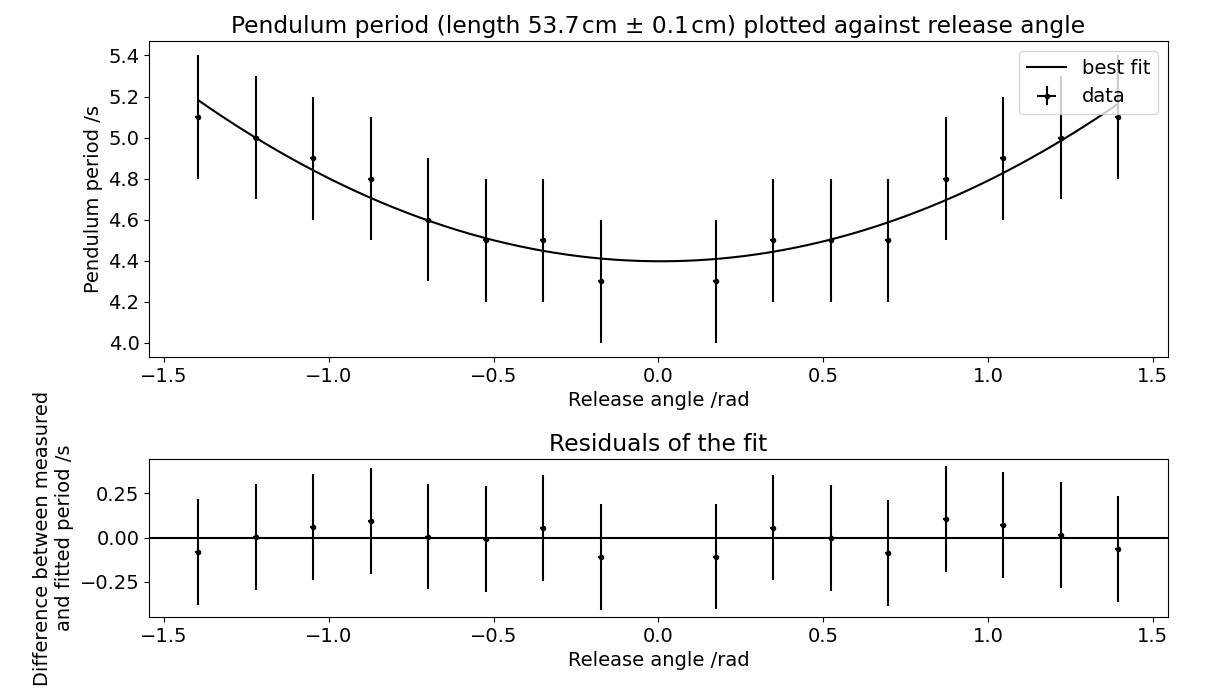
\includegraphics[width=\textwidth]{../figures/period_vs_release_angle.png}
    \caption{\centering Period plotted against release angle}
    \label{fig:figure 2}
\end{figure}

All data collected for this graph were done without the need for tracking software. The uncertainty for the protractor was taken to be the smallest increment, $0.5^{\circ}$ converted to radians, and the period uncertainty was taken to be the average human reaction time, $0.25\,\text{s}$ \cite{reaction-time}.

\subsection{Analysis}
According to Section \ref{Background}, if $-20^{\circ} \lesssim \theta \lesssim 20^{\circ}$, then a linear line of best fit would be expected, which matches the trends generated by the graph.

Since the data collected contained angles ranging from $ 80^{\circ} \leq \theta \leq 80^{\circ}$, a quadratic power series fit modelled by the equation:
\begin{equation}
    T_0(1 + B\theta_0 + C\theta_0^2)
\end{equation}
where $T_0$ represents the period, $\theta_0$ the release angle and $B$ and $C$ some arbitrary constants would pass through more error bars and leave smaller overall residuals than a linear fit. Thus, it can be concluded that the pendulum's period depends on amplitude, which becomes more apparent for larger angles.

Lastly, the residuals shown on the graph do not suggest much asymmetry regarding the pendulum as the negative release angles appear symmetrical when compared to positive release angles. However, a single-stringed pendulum tends to spin in an elliptical fashion when released, affecting accurate measurements.

\section{Finding the Q Factor}

\subsection{Experimental Setup}
In order to correct for potential asymmetry and elliptical orbit, a degree of freedom was removed from the pendulum by threading a string through the stainless steel quick link and fastening the 2 strings in 2 locations to form the shape of a ``V''. Then pendulum would then swing back and forth in the plane perpendicular to the ``V'', and the tendency for each string to balance out the load prevents it from swinging in any other direction. Additionally, the pendulum was kept the same length as the previous setup (perpendicular distance from threading location to top of desk), and extra precautions were taken to make sure the pendulum was symmetrical along the vertical axis. Below is a setup of what was described above:
\begin{figure}[!hptb]
    \centering
    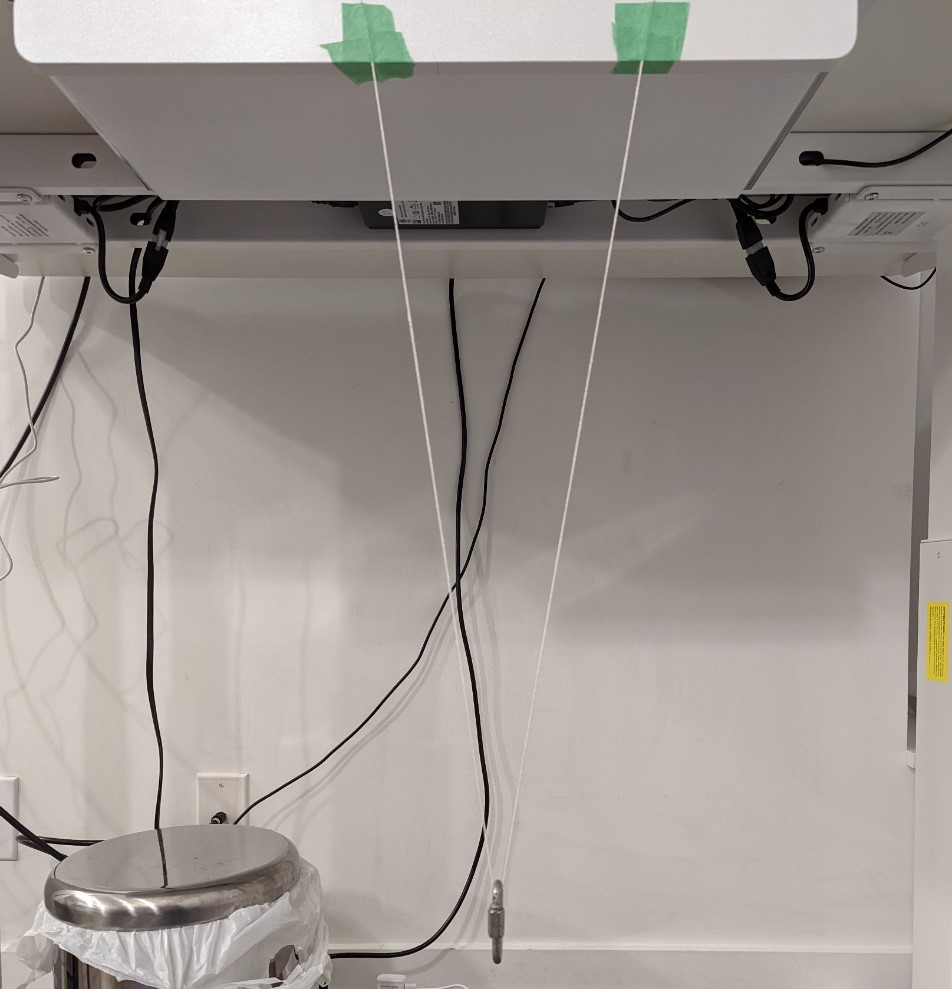
\includegraphics[width=0.5\textwidth]{../figures/exp_setup2.jpg}
    \caption{\centering Improved version of the pendulum used to determine Q factor}
    \label{fig:figure 3}
\end{figure}

\newpage

\subsection{Data}
Due to the double-string contraption, the camera must be positioned in a place where the chance of capturing both strings in the same frame is minimized.

A protractor was not included in the experimental setup this time because Tracker \cite{tracker} was used to measure the angles. First, data was collected such that the maximum amplitude of the pendulum could be plotted against time:

\begin{figure}[!hptb]
    \centering
    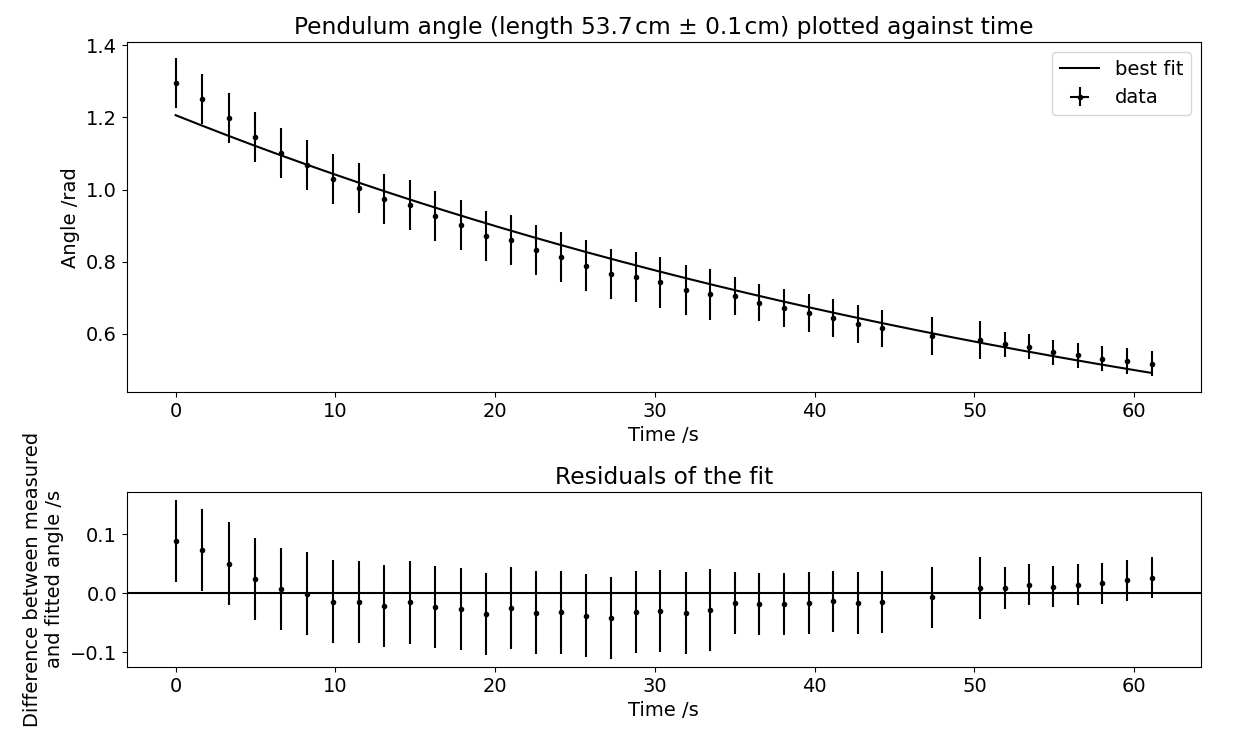
\includegraphics[width=\textwidth]{../figures/max_amplitude_vs_time.png}
    \caption{\centering Graph of maximum amplitude vs. time}
    \label{fig:figure 4}
\end{figure}

The uncertainty for time was taken to be $1/f$ where $f$ represents the frame rate of the video imported into Tracker, namely $120\,\text{fps}$. The uncertainty for angle was calculated this time for each individual maximum by taking half the range of the sweeping area that the string made in Tracker due to video blur.

\subsection{Analysis}
The exponential fit used to create a curve of best fit for the data was taken from Equation \ref{eq:eq3}, removing the periodic motion portion. The equation for the fit is equal to:
\begin{equation}
    1.21e^{-{t}/68}
\end{equation}

With this information and also knowing the period ($1.67\,\text{s}$) of the pendulum when the release angle is $1.2064\,\text{rad}$, the $Q$ factor can be calculated. The uncertainty of the $Q$ factor is taken to be the largest percent uncertainty of $\tau$ and $T$.

$\tau$ was calculated to have an uncertainty of 1, which is less than the percent uncertainty of $T$, taken to be $0.3/1.67 \approx 15\%$. Thus, the value of $Q$ can be calculated to be $130 \pm 20$.

However, Graph \ref{fig:figure 4} can also be used to find the Q factor by counting the number of oscillations. Since the total amplitude does not decrease down to $e^-\pi \%$ of the original amplitude, it suffices to calculate a value for $Q/5$. The closes data points above and below $\theta_0e^{-{pi/5}}$ correspond to the $24^\text{th}$ and $25^\text{th}$ swing. Multiplying these values by 5 and taking half the difference (range) to be the uncertainty gives another Q factor of $123 \pm 2$.

\newpage

\printbibliography

\end{document}
